\section{Introduction/Review}
The details and proofs of most things in this section can be found in my MAT354 notes \href{http://individual.utoronto.ca/rishibhp/notes/MAT354_notes.pdf}{here}.

\subsection{Holomorphic Functions}
If $f(z)$ is a complex-valued function on the complex numbers, we say $f$ is \textit{holomorphic} if
$$\lim_{h \to 0} \frac{f(z + h) - f(z)}{h}$$
exists. Suppose we call the limit $c$.
Then the above condition is equivalent to saying there exists some $\phi(h)$ such that
$$f(z + h) = f(z) + ch + \phi(h)h$$
where $\lim_{h \to 0} \phi(h) = 0$.

We can identify $\C$ with $\R^2$ and consider what conditions it places on the derivatives (in the real sense). So suppose we have $c = (a, b)$ and $h = (\xi, \eta)$. Then the map $ch$ becomes $(a + ib)(\xi + i \eta) = a\xi - b\eta + i(b \xi + a \eta)$. In terms of the real variables, we can write
$$\matrix{\xi \\ \eta} \mapsto \matrix{a & -b\\b & a} \matrix{\xi \\ \eta}$$
The matrix is the differential of $f$. Thus looking at the columns we see the following equation is satisfied
$$\frac{\partial f}{\partial x} + i \frac{\partial f}{\partial y} = 0$$
This is known as the Cauchy-Riemann equation(s). If we write $f = u + iv$, we can again use the matrix to get
\begin{align*}
    \frac{\partial u}{\partial x} &= \frac{\partial v}{\partial y}\\ 
    \frac{\partial u}{\partial y} &= -\frac{\partial v}{\partial x} 
\end{align*}
which are another way of formulating the Cauchy-Riemann equations.

Recall that if $f$ is differentiable, we have
$$df = \frac{\partial f}{\partial x}dx + \frac{\partial f}{\partial y}dy$$
This means that for the identity map $z = x + iy$ we have
\begin{align*}
    dz &= dx + idy\\
    d\ol{z} &= dx - idy
\end{align*}
We can then solves for $dx$ and $dy$ to get
\begin{align*}
    dx &= \frac{1}{2}(dz + d\ol{z})\\
    dy &= \frac{1}{2i}(dz - d\ol{z})
\end{align*}
Thus we get
$$df = \frac{1}{2}\left( \frac{\partial f}{\partial x} - i \frac{\partial f}{\partial y} \right)dz + \frac{1}{2} \left( \frac{\partial f}{\partial x} + i \frac{\partial f}{\partial y} \right) d \ol{z}$$
This motivates us to define
\begin{align*}
    \frac{\partial}{\partial z} &= \frac{1}{2} \left( \frac{\partial}{\partial x} - i \frac{\partial}{\partial y} \right)\\
    \frac{\partial}{\partial \ol{z}} &= \frac{1}{2} \left( \frac{\partial}{\partial x} + i \frac{\partial}{\partial y} \right)
\end{align*}
One thinks of these as the duals to $dz$ and $d\ol{z}$. With this notation we can once again rewrite the Cauchy-Riemann equations to 
$$\frac{\partial f}{\partial \ol{z}} = 0$$
Roughly speaking, this says that a holomorphic function should only depend on $z$ and not $\ol{z}$.

\subsection{Harmonic functions}
Apart from holomorphic functions, another important class of functions are the harmonic functions.
\begin{definition}[Harmonic functions]
A real- or complex-valued function $f(x, y)$ is said to be \textit{harmonic} if it is $C^2$ and
$$\frac{\partial^2 f}{\partial x^2} + \frac{\partial^2 f}{\partial y^2} = 0$$
\end{definition}

The operator
$$\Delta := \frac{\partial^2}{\partial x^2} + \frac{\partial^2}{\partial y^2}$$
is often called the Laplacian. It is easy to verify from the definition that if a complex-valued function is harmonic then so are its real and imaginary parts. Using the definitions of $\frac{\partial}{\partial z}$ and $\frac{\partial}{\partial \ol{z}}$ we get
$$\Delta = 4\frac{\partial^2}{\partial z \partial \ol{z}}$$
This immediately implies that holomorphic functions are harmonic since they satisfy $\frac{\partial f}{\partial \ol{z}}$ is 0, which also means that the real and imaginary parts of a holomorphic function are harmonic. In fact the relationship between harmonic and holomorphic functions runs deeper than that. Any real-valued harmonic function is locally the real part of a holomorphic function, which is uniquely determined up to the addition of a constant (shown in \autoref{subsec:harmonic-func-revisit}). The holomorphic function need not be define globally. An example of a harmonic function whose associated holomorphic function is only locally defined is $\log(\abs{z})$. This is harmonic on $\C \setminus \{0\}$ but the corresponding holomorphic function would have to be $\log(z)$ which does not have a holomorphic branch on the entire punctured plane.

\subsection{Geometric Models}
We are often interested in the behaviour of holomorphic functions at $\infty$ to the extent that we often include it in our domain. If we add the point at infinity to $\C$ we get $\C \cup \{\infty\}$ the extended complex plane. Two primary ways of modelling this space are the Riemann sphere and one-dimensional complex projective plane (which we will see are equivalent).

Recall that the plane is homeomorphic to the sphere without a point. Thus if we add a point to the plane (namely the point at infinity) we get exactly a sphere. We can cover the sphere using two charts via stereographic projection. For example we have the homeomorphism $S^2 \setminus \{N\}$
\begin{align*}
    S^2 \setminus \{N\} &\to \C\\
    (x, y, t) &\mapsto z := \frac{x + iy}{1 - t}
\end{align*}
The point at infinity then is the north pole. We can cover this point by stereographic projection from the south pole where the chart is given by
\begin{align*}
    S^2 \setminus \{S\} &\to \C\\
    (x, y, t) &\mapsto z' := \frac{x - iy}{1 + t}
\end{align*}
If we just wanted a chart, we would use $\frac{x + iy}{1 + t}$ which is the usual projection from $S^2\setminus \{S\}$. But since we want to impose a complex structure on $S^2$ we want the transition maps to the holomorphic so we take the complex conjugate instead. Note that with the above choice we have
$$zz' = \frac{x + iy}{1 - t} \cdot \frac{x - iy}{1 + t} = \frac{x^2 + y^2}{1 - t^2} = 1$$
This means that $z' = \frac{1}{z}$ which allows us to translate to coordinates at infinity. For example, given a map $f$ which is defined on the complement of a (large) disk, we say $f$ is holomorphic at $\infty$ if $f(\frac{1}{z})$ is holomorphic at $0$.

A seemingly different but ultimately equivalent geometric model is the one dimensional complex projection space. Define $P^1(\C) := \C^2 \setminus \{0\}/\sim$ where $(x_0, x_1) \sim (y_0, y_1)$ if and only if there is some non-zero complex number $\lambda$ such that $(x_0, x_1) = \lambda (y_0, y_1)$. Let $[x_0, x_1]$ denote the equivalence class of $(x_0, x_1)$.

Once again we can cover this space with two coordinate charts. For $i = 0$ and $i = 1$ we define $U_i := \{[x_0, x_1] \in P^1(\C) : x_i \neq 0\}$. Then we can define charts
\begin{align*}
    U_0 &\to \C\\
    [x_0, x_1] &\mapsto z := \frac{x_1}{x_0}
\end{align*}
and
\begin{align*}
    U_1 &\to \C\\
    [x_0, x_1] &\mapsto z' := \frac{x_0}{x_1}
\end{align*}
These are well-defined due the equivalence placed upon the point. These are both homeomorphisms onto $\C$. Once again we see that $zz' = 1$. This means that $P^1(\C)$ is obtained by gluing two copies of $\C$ along the complement of the origin by the formula $z' = \frac{1}{z}$, exactly like we had with the sphere.

\subsection{Cauchy's Theorem}
Much of complex analysis is about studying the properties of holomorphic functions and one of the fundamental results in this area is Cauchy's Theorem. Before we get to the theorem, we should maybe establish some basis facts about (differential) forms.

\begin{figure}[ht]
    \centering
    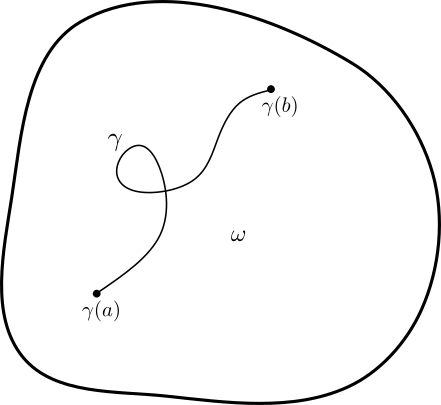
\includegraphics[scale=0.85]{Images/integrating_forms.png}
    \caption{We integrate the 1-form $\omega$ over the curve $\gamma$}
    \label{fig:integrating-forms}
\end{figure}

Given an open set (of $\C$) $\Omega$, a differential form on $\Omega$ is $\omega = Pdx + Qdy$ with $P, Q$ continuous functions (taking values in $\C$) on $\Omega$. We can integrate a form along a piecewise $C^1$ curve $\gamma: [a, b] \to \Omega$ by the formula
\begin{align*}
    \int_\gamma \omega = \int_a^b f(t) dt
\end{align*}
where
$$f(t) := P(x(t), y(t))x'(t) + Q(x(t), y(t)) y'(t)$$
We see this by computing the pullback of $\omega$ by $\gamma$. The reason we integrate forms and not functions is because then the integral is independent of how we parameterise the curve (in order to verify this we simply use integration by substitution).

Now suppose we are given a form $\omega$ and suppose there exists a function $F$ so that
$$\omega = dF = \frac{\partial F}{\partial x}dx + \frac{\partial F}{\partial y}dy$$
Then we call $F$ a \textit{primitive} of $\omega$. If $\omega$ has a primitive then
\begin{align*}
    \int_\gamma \omega &= \int_\gamma \frac{\partial F}{\partial x}dx + \frac{\partial F}{\partial y}dy\\
    &= \int_a^b \frac{\partial F}{\partial x}d(x(t)) + \frac{\partial F}{\partial y}d(y(t)) dt\\
    &= \int_a^b (F \circ \gamma)'(t) dt\\
    &= F(\gamma(b)) - F(\gamma(a))
\end{align*}

It is clear then, that if $\gamma$ is any closed curve (i.e. $\gamma(a) = \gamma(b)$) then $\int_\gamma \omega = 0$ provided that $\omega$ has a primitive. In fact the converse is also true.
\begin{theorem}
A form $\omega$ on a connected open set $\Omega$ has a primitive if and only if the integral of $\omega$ over any closed curve is 0.
\end{theorem}
\begin{proof}
We choose a basepoint $(x_0, y_0) \in \Omega$. Then we define the primitive $F(x, y)$ by integrating along a path from $(x_0, y_0)$ to $(x, y)$. This is well-defined due to the fact that the integral over closed curves is 0 and one can verify that indeed defined this way, we have $dF = \omega$. The details can be found in Proposition 9.2 in my MAT354 notes \href{http://individual.utoronto.ca/rishibhp/notes/MAT354_notes.pdf}{here}. 
\end{proof}

If we have a disk, then it is much easier to check whether or not a form has a primitive. Namely, a form has a primitive if and only if the integral over the boundary of any rectangle (by which we mean a rectangle whose sides are parallel to the axes) is 0. This is simply because in a disk, we can connect any point to the center via paths that run parallel to the axes (for example we first travel only in the $x$-direction and then only in the $y$-direction). Thus although the existence of a primitive might be difficult to check globally, it is fairly straightforward to do locally. This inspires the following definition.

\begin{definition}[Closed forms]
    We say a form $\omega$ is closed if the integral over the boundary of any (small) rectangle is 0.
\end{definition}
By the above discusssion, this is equivalent to saying that $\omega$ has a local primitives. Moreover, if the integral over the boundary of small rectangles is 0, then the integral over the boundary of any rectangle is 0 since any rectangle can be cut into smaller rectangles.

Importantly, however, closed forms need not have a primitive. The classic example of a form which has local primitives but not global ones is 
$$ \omega = \frac{dz}{z}$$
defined on $\C \setminus \{0\}$. Local primitives are easy to find since these are just branches of $\log(z)$. However $\omega$ cannot have a global primitive since the integral over the unit circle is not zero. If we define $\gamma(\theta) = e^{i \theta}$ for $\theta \in [0, 2\pi]$ then
$$\int_\gamma \omega = \int_0^{2\pi} \frac{i e^{i\theta}}{e^{i \theta}} d\theta = 2\pi i$$

Now we can state and prove Cauchy's theorem.
\begin{theorem}[Cauchy's Theorem]
    If $f(z)$ is holomorphic then the differential form $f(z) dz$ is closed.
\end{theorem}
\begin{proof}
    Once again, the proof can be found in my \href{http://individual.utoronto.ca/rishibhp/notes/MAT354_notes.pdf}{MAT354 notes} under Theorem 9.5.
\end{proof}
\begin{remark}
In Cauchy's Theorem, it is enough to assume that $f$ is continuous on $\Omega$ and holomorphic everywhere except possibly on a line.
\end{remark}

\begin{corollary}
Holomorphic functions $f(z)$ locally have a holomorphic primitive.
\end{corollary}
\begin{proof}
    We have seen above that $f(z)dz$ has a primitive. Now we show that the primitive is in fact holomorphic. Suppose the primitive is given by $F$. Then
    \begin{align*}
    f(z)dz = dF = \frac{\partial F}{\partial z}dz + \frac{\partial F}{\partial \ol{z}} d\ol{z}
    \end{align*}
    Since $dz, d\ol{z}$ form a basis they are in particular linearly independent which means that $\frac{\partial F}{\partial \ol{z}}$ must be 0.
\end{proof}